\section{Weather Monitoring System 2.0}
\subsection{Neuerungen} % WMS
Das mit dem Namen ,,WMS 2.0'' betitelte Projekt vereint die in dieser Arbeit genannten
Programme, Algorithmen und Oberflächen in einer Software und implementiert diese komplett
in der Sprache Go bzw. Golang (für Go-Language) mit allen im Nachhinein realisierten
Optimisierungsansätzen und neuen Funktionen durch eine Verknüpfung bestehender Software.\\
Das entstandene System ist in der Lage alle Aufgaben von ViSys zu erfüllen, allerdings durch
eine native Ausgabe in HTML ist das ,,stylen'' der Ausgabe um ein vielfachen einfacher und
anschaulicher. Alle Zwischenergebnisse und Daten aus den verschiedenen Quellen können durch
die Unterstützung von Kohärenz (Parallelismus) von Golang analysiert, verglichen, aktualisiert
und abgespeichert werden.\\
Das Resultat ist ein platformunabhängiger Webserver, welcher nicht mehr von Apache oder PHP
abhängig ist, und direkt Quellenabgleich und Ausgabe vereint. Dieser implementiert das REST-Ful
Paradigma, funktioniert also auf minimalen Speicher und CPU Anspruch. \\
Eine Datenbankstruktur, ähnlich der die in WMS 1.0 für die Admin Konten benutzt wird,
wird simuliert und gibt Nutzern personalisierte Funktionen.
Das Erstellen eigener WMS-Slideshows, wie sie im Foyer der Schule Anwendung finden
ist somit möglich. Als Quelle der Grafiken können die Wetterdaten, verknüpft mit einem
Stylesheet, ausgewählt werden, aber der Nutzer kann auch selbst Grafiken für seine eigene
Slideshow hochladen. Er erhält schließlich einen Link für seine eigene Fullscreen Slideshow
mit immer aktuellen Daten, nach seiner Auswahl.\\
Auch die Ausgabe der puren Daten ist in Form von Tabellen oder ASCII Text möglich und
erlaubt die Weiterverwendung in anderer Software.

\subsection{HTTP-Handler} % WMS
Es musste ein dedizierter HTTP-Handler in Golang geschrieben werden. Bei der Implementation
wird die Cache benutzt und Abfragen für Wetterdaten werden zwischengespeichert. Das heißt bei der
Nachfrage von Daten durch einen Nutzer müssen nicht immer die Quellen über das Netzwerk befragt werden. 
Der Server speichert selbst die aktuellen vorhandenen Daten, 
vergleicht diese auf Lücken im Datensatz. 
Sollten Daten nicht vorhanden sein, oder sind Daten einer Quelle
älter als 15 Minuten, werden die Daten von den Quellen asynchron im Hintergrund nachgeladen.\\

\subsection{Ausgabeformate}
Die neuen Ausgabeformate sind die Anforderungen, die dazu geführt haben, dass ein neues Programm
entwickelt werden musste. Die erste Priorität war es die Daten der Seewetterstation Kühlungsborn
durch Modellergebnisse zu ergänzen um beschädigtes Equipment zu ersetzen und die Ausgabe in Textform
für die TSK zu automatisieren.\\
Dieses Ausgabeformat wird durch die Subroutine ,,aktuelltxt'' behandelt, benannt nach der Datei aktuell.txt
die von der TSK abgefragt wird. Die bestehende Syntax der Datei musste durch die neue Quelle gefüllt
werden. Das Ergebnis konnte direkt eingesetzt werden.\\
\lstinputlisting[language=bash]{example/aktuell.txt}
Sofern kein Fehler festgestellt wird, wird als Quelle OpenWeatherMap.org benutzt. Ansonsten kann auf
YahooWetter zurückgefallen werden.\\
Die TSK möchte des weiteren auch auf eine ASCII Wetterprognose zugreifen. Diese wird ähnlich wie die
,,Messdaten'' Datei erzeugt. Die Erstellung ist allerdings noch experimentell.
\lstinputlisting[language=bash]{example/prognose.txt}
Diese Daten werden über die neue Weboberfläche angeboten. Die Beta Versionen
laufen auf der Domain \link{http://viwetter.de/wms/} im Internet auf dem master Branch der
Entwicklung.\\
Dort ist auch der neue Stylesheet des Interfaces eingebunden. Das Interface
ist nun benutzerfreundlicher, und auch für die Anwendung auf dem Mobiltelefon und Tablet optimiert.\\
Hier ist die Designseite zu sehen, diese ist gefüllt mit Lorem Ipsum Text.
\begin{center}
    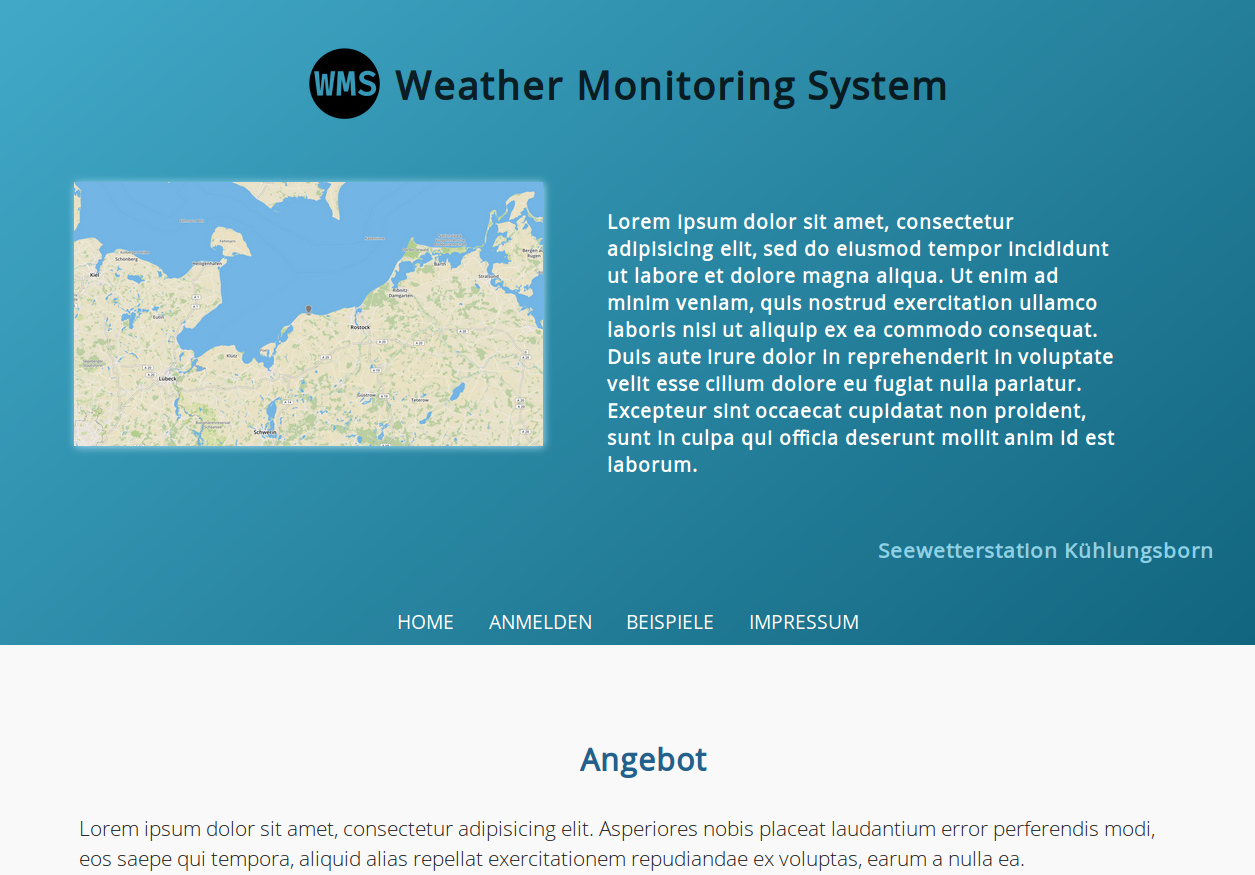
\includegraphics[width=\linewidth]{imgs/wms20.png}
\end{center}
Ohne Benutzerkonto ist auf der Seite allerdings zum aktuellen Zeitpunkt noch
nicht viel offen ersichtlich, auch der Quelltext ist zum Teil Closed-Source.
Die hier gezeigten Teile sind allerdings auf GitHub gespiegelt unter
\link{https://github.com/eixmb/aktuelltxt}.


\subsection{Kontensystem und kommerzielle Nutzung}
Die Zukunft von WMS 2.0 sieht vor, das Nutzer in Form von verschiedenen Ebenen von
Abonnements auf die Oberfläche zugreifen können.\\
Jeder Nutzer kann dann seine eigenen Slideshows wie im alten WMS 1.0 einstellen.
Zur Auswahl für die anzuzeigenden Daten stehen dem privaten Nutzer dann Wetterdaten
in Form von Tabellen, Funktionsgraphen und Säulen- bzw. Balkendiagrammen. Diese
können durch die Einbindung als HTML sogar durch JavaScript animiert werden. \\
Weitere Formate sind die ,,Wussten sie schon'' Slides die auch in den Schul-WMS Anzeigen
eingestellt werden, automatisiert erzeugte Bodenwetterkarten mit ausgewerteter Prognose,
sowie die vom Nutzer hoch geladenen Grafiken.
Firmennutzer können dann noch eigene Werbeanzeigen zwischen den Grafiken schalten.

\subsection{Entwicklung} % WMS
Die Sprache Golang lässt eine Organisierung von Quelltext in Paketen zu. Diese können dann in
anderen Paketen importiert werden. Es gibt auch das Äquivalent zu public und private, wobei in
Golang der Fokus auf dem schreiben von Software, welche in mehreren Prozessen gleichzeitig ausgeführt liegt.
Dieses Paradigma wird hauptsächlich durch die Benutzung von sog. Channels erreicht. Channels sind FIFO
Buffer mit festgelegter Größe. Sie sind Programmfluss blockierend, wenn sie voll sind, bzw. nicht als Buffer
initialisiert wurden. Durch Channels ist es möglich in dem Programm die Daten an die einzelnen Nutzer asynchron
weiterzugeben, indem jede Anfrage nach einer Ausgabe (egal welcher Form), als Funktion in einem Channel an
einen sog. Worker weitergegeben wird.\\
Die Worker überprüfen dann nebeneinander die Aktualität der Daten und führen auch durch einen Mutex geschützt
Aktualisierungen durch. So kann sicher gegangen werden, dass Daten nicht korrupiert werden und nicht mehrmals die
selbe Nachfrage an die Quellen geschickt wird.\\
Die Worker antworten schließlich, nachdem sie die Aufgabe der ihnen übergebenen Funktion erfüllt haben mit einer
HTML-Response, die an den Client geschickt wird.
